\section{The Chromatic Number Problem}\label{sec:chromatic}

This section investigates the various well-known methods to either estimate or find the exact chromatic number for
a graph.  Since the chromatic number problem is NP-hard, an alternative to finding an exact answer is finding lower
and upper bounds for the actual value.  If these bounds happen to match then they provide the actual chromatic
number.  Algorithms that find the exact chromatic number are of the branch-and-bound variety.  The two most
well-known algorithms are one proposed by Christofides~1971~\cite{christofides} with modifications by
Wang~(1974)~\cite{wang} and the so-called Zykov algorithms, with a particular implementation by Corneil and
Graham~(1973)~\cite{corneil}.

The specifics of the random graph analysis used throughout this research are described in detail in
\sectionname~\ref{sec:random}.  In short, a binomial edge probabity model was used.  Trials were run for edge
probabilities from \(p=10\%\) to \(p=90\%\) in steps of \(10\%\).  For P-time algorithms, \(1000\) trials were run
for each edge probability and for each order from \(n=5\) to \(n=50\).  For non-P-time algorithms, due to increased
runtime duration, the maximum order was reduced to \(30\) and the number of trials was reduced to \(100\) for
\(n\ge20\).

\subsection{Finding a Lower Bound}\label{sec:sub:lower}

The most popular strategy for estimating a lower bound for the chromatic number of a graph is based on the
statement of \propname~\ref{prop:clique}.  For a graph \(G\):
\[\w'(G)\le\w(G)\le\X(G)\]
where \(\w'(G)\) is a lower bound estimate for the clique number of \(G\).  Another less popular bound is given by
\theoremname~\ref{thm:lbalpha}~\cite{chartrand}.

\begin{theorem}
  \label{thm:lbalpha}
  Let \(G\) be a graph of order \(n\).  \(\displaystyle \X(G)\ge\frac{n}{\a(G)}\).
\end{theorem}

\begin{proof}
  Assume that \(G\) is \chromatic{k}.  This means that \(V(G)\) can be partitioned into \(k\) non-empty independent
  sets \(A_1,\ldots,A_k\), where each \(\abs{A_i}\le\a(G)\).
  \[n=\abs*{\bigcup_{1\le i\le k}A_i}=\sum_{i=1}^k\abs{A_i}\le\sum_{i=1}^k\a(G)=k\a(G)\]
  Therefore, \(\displaystyle k\ge\frac{n}{\a(G)}\).
\end{proof}

Note that both of the above lower bounds are tight when \(G\) is empty or complete and are related by the statement
of \theoremname~\ref{thm:isclique}:
\[\w(G)=\a(\bar{G})\]

\subsubsection{The Mycielski Construction}\label{sec:sub:sub:mycielski}

It is well-known that certain triangle-free graphs with \(\w(G)=2\) can have arbitrarily high \(\X(G)\).  Examples
are the graphs created using the so-called \emph{Mycielski} construction~\cite{west}:
\begin{enumerate}
\item Start with \(G=P_2\) \((\X(G)=2)\).
\item\label{step:myc:repeat} For the vertices in \(v\in V(G)\), create new vertices \(U=\set{u_1,\ldots,u_n}\) such
  that \(N(u_i)=N(v_i)\).  The new vertices form what is referred to as a \emph{shadow} graph.
\item Add an additional vertex \(w\) such that \(N(w)=U\) and call this new graph \(G'\), which has
  \(\X(G')=\X(G)+1\).
\item Let \(G=G'\) and go to step~\ref{step:myc:repeat}.
\end{enumerate}

The first three graphs resulting from the Mycielski construction are shown in \figurename~\ref{fig:mycielski}.

\begin{figure}[H]
  \begin{minipage}{1in}
    \centering
    \scalebox{0.75}{
      \begin{tikzpicture}[every node/.style={labeled node}, node distance=1in]
        \pathV{\(v_1\),\(v_2\)}{(0,0)}{below};
      \end{tikzpicture}
    }

    \(k=2\)
  \end{minipage}
  \begin{minipage}{2in}
    \centering
    \scalebox{0.75}{
      \begin{tikzpicture}[every node/.style={labeled node}, node distance=1in]
        \cycleV{\(v_1\),\(v_2\),\(u_1\),\(w\),\(u_2\)}{(0,0)}{0.75in}{90}{};
      \end{tikzpicture}
    }

    \(k=3\)
  \end{minipage}
  \begin{minipage}{2.75in}
    \centering
    \scalebox{0.75}{
      \begin{tikzpicture}[every node/.style={labeled node}, node distance=1in]
        \cycleV{\(v_1\),\(v_2\),\(v_3\),\(v_4\),\(v_5\)}{(0,0)}{1.25in}{90}{o};
        \cycleV{\(u_1\),\(u_2\),\(u_3\),\(u_4\),\(u_5\)}{(0,0)}{0.75in}{90}{i};
        \draw (i1) edge (o5) edge (o2);
        \draw (i2) edge (o1) edge (o3);
        \draw (i3) edge (o2) edge (o4);
        \draw (i4) edge (o3) edge (o5);
        \draw (i5) edge (o4) edge (o1);
        \node (w) at (0,0) {\(w\)};
        \draw (w) edge (i1) edge (i2) edge (i3) edge (i4) edge (i5);
      \end{tikzpicture}
    }

    \(k=4\)
  \end{minipage}
  \caption{The first three graphs from the Mycielski construction.}
  \label{fig:mycielski}
\end{figure}

The third graph in \figurename~\ref{fig:mycielski} is called the \emph{Gr\"otzsch} graph.  For another example of
triangle free graphs with arbitrarily high chromatic number, see Zhang~\cite{zhang}.  Nevertheless, for the general
case the clique number is a suitable lower bound for the chromatic number.

\subsubsection{The Edwards Elphick Algorithm}\label{sec:sub:sub:edwards}

Unfortunately, the clique number problem for a graph \(G\) is also NP-hard, so the next best step is to use a
P-time calculation for a \(\w'(G)\) that is as tight as possible to the actual \(\w(G)\).  Edwards and
Elphick~(1982)~\cite{edwards} investigated several such methods and concluded that the best method was a simple
calculation based on the adjacency matrix of \(G\):
\begin{enumerate}
\item Select (either lowest index or at random) a vertex \(v\in V(G)\) of maximum degree in \(G\)
  \((\deg(v)=\dmax(G))\) and let \(S=\set{v}\).
\item\label{step:edw:select} Select the vertex \(v_i\in V(G)\) such that \(v_i\notin S\) and with the minimum index
  value \(i\) that is adjacent to all of the vertices in \(S\).  If no such vertex exists then go to
  step~\ref{step:edw:done}.
\item Add \(v_i\) to \(S\) and go to step~\ref{step:edw:select}.
\item\label{step:edw:done} \(G[S]\) is a complete subgraph of \(G\) so conclude that \(\w'(G)=\abs{S}\le\w(G)\).
\end{enumerate}

The results of a random graph analysis of the Edwards Elphick algorithm measuring the mean of \(\w(G)-\w'(G)\) are
shown in \figurename~\ref{fig:edwards1:error}.  The error generally increases with both edge probability and order;
however, there appears to be a small hitch in the curves between \(p=80\%\) and \(p=90\%\) for orders \(n\le40\).
This may be because of the increased probability that the next selected vertex is in fact universal.

\begin{figure}[H]
  \centering
  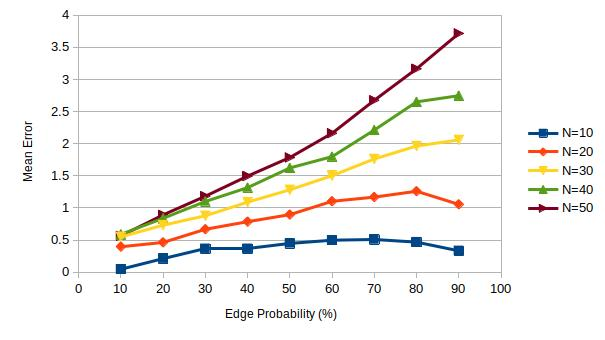
\includegraphics[width=5in]{edwards1_error}
  \caption{Edwards Elphick algorithm mean error.}
  \label{fig:edwards1:error}
\end{figure}

The mean number of steps is shown in \figurename~\ref{fig:edwards1:steps}.  The number of steps increases with both
edge probability and order, so the worst case for each order is assumed to be at \(P=90\%\).

\begin{figure}[H]
  \centering
  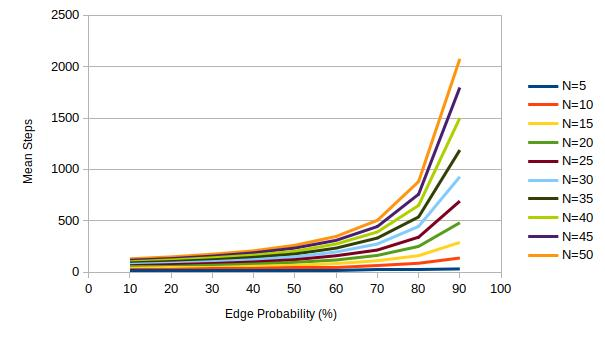
\includegraphics[width=5in]{edwards1_steps}
  \caption{Edwards Elphick algorithm mean number of steps.}
  \label{fig:edwards1:steps}
\end{figure}

A graph of the \(P=90\%\) values for each order is shown in \figurename~\ref{fig:edwards1:runtime}.  Note that the
runtime complexity is \(\BO(n^2)\) as expected.  Thus, the Edwards Elphick algorithm would be suitable for use as a
lower bound approximator step in a branch-and-bound algorithm.

\begin{figure}[H]
  \centering
  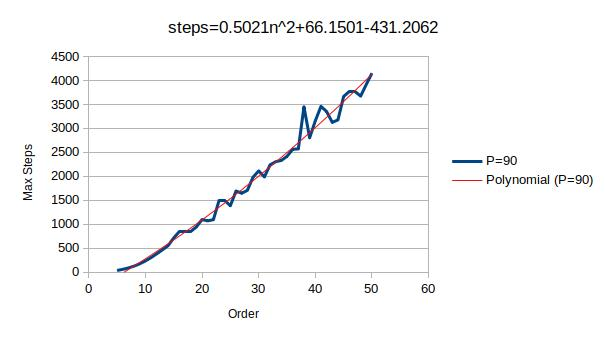
\includegraphics[width=5in]{edwards1_runtime}
  \caption{Edwards Elphick algorithm runtime complexity.}
  \label{fig:edwards1:runtime}
\end{figure}

Step~\ref{step:edw:select} of the Edwards Elphick algorithm selects the next vertex of lowest index that is
adjacent to all previously selected vertices.  An improvement would be to select a vertex with the highest degree
that is adjacent to all previously selected vertices.  This would of course increase the average runtime complexity
to the worst case of the unimproved algorithm, but it should still be P-time.  The results of this improved
algorithm are shown in \figurename~\ref{fig:edwards2:error}.  Note that the improved algorithm cuts the mean error
in half.  Also note that the hitch at \(p=80\%\) remains and is more pronounced, probably due to the increased
probability of finding a high degree vertex that is more likely to be part of a clique.

\begin{figure}[H]
  \centering
  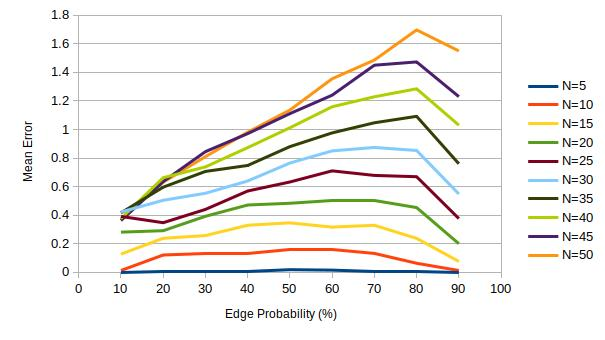
\includegraphics[width=5in]{edwards2_error}
  \caption{Improved Edwards Elphick algorithm mean error.}
  \label{fig:edwards2:error}
\end{figure}

The increase in the number of steps is demonstrated in \figurename~\ref{fig:edwards2:steps}.

\begin{figure}[H]
  \centering
  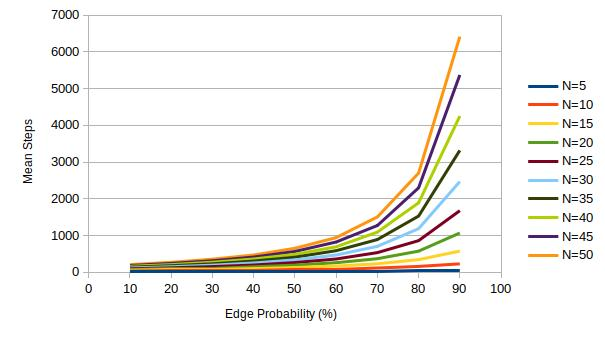
\includegraphics[width=5in]{edwards2_steps}
  \caption{Improved Edwards Elphick algorithm mean number of steps.}
  \label{fig:edwards2:steps}
\end{figure}

And the new runtime complexity approximation is shown in \figurename~\ref{fig:edwards2:runtime}.  The improved
algorithm is still \(\BO(n^2\).

\begin{figure}[H]
  \centering
  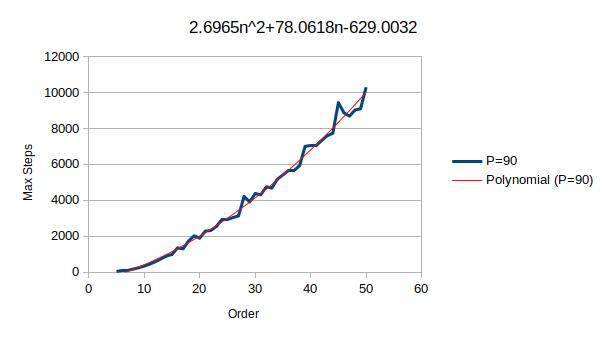
\includegraphics[width=5in]{edwards2_runtime}
  \caption{Improved Edwards Elphick algorithm runtime complexity.}
  \label{fig:edwards2:runtime}
\end{figure}

\subsubsection{The Bron Kerbosch Algorithm}\label{sec:sub:sub:bron}

Although an estimate of the clique number is nice, an exact value is better.  Unfortunately, the clique number
problem is also NP-hard.  A nice summary of well-known exact clique number algorithms is given by Xiao and
Nagamouchi~(2017)~\cite{xiao}.  They claim that the known algorithms tend to converge on a runtime complexity of
\(\BO(1.2^n)\).  These algorithms tend be somewhat complex and geared towards larger \(n\).

A simpler yet efficient alternative to these exact algorithms for more modest values of \(n\) is the Bron Kerbosch
(BK) algorithm~(1973)~\cite{bron}.  In fact, the algorithm that was incrementally developed in
\sectionname~\ref{sec:sub:bandb} is essentially the BK algorithm.  The advantage of BK is that it finds all
possible cliques in a graph, and hence can be used to find \(\a(G)=\w(\bar{G})\).  Moon and
Moser~(1965)~\cite{moon} show that every graph \(G\) of order \(n\) has at most \(3^{\frac{n}{3}}\) maximal
cliques, so the runtime complexity of the Bron Kerbosch algorithm is expected to be about \(\BO(1.44^n)\).

The heart of BK is a recursive subroutine called \emph{extend} that implements the breadth of a level in the
corresponding state tree, and recursively calls itself in order to implement the branches in the state tree.
At each node in the state tree, three vertex lists are maintained:

\begin{description}
\item[compsub] The current maximal clique accumulator.
\item[candidates] A set of vertices that can be added to \emph{compsub}.
\item[used] A set of vertices that already have been used in previous branches.
\end{description}

The initial call is seeded with an empty \emph{compsub} and all of the graph's vertices in \emph{candidates}.  Each
call to \emph{extend} performs the following steps:
\begin{enumerate}
\item\label{step:bron:check} If \emph{used} contains a vertex that is adjacent to everything in \emph{candidates}
  then any generated cliques in the current subtree will never be maximal, so return.  This implements the
  non-maximal bounding condition.
\item\label{step:bron:select} The next vertex is selected from \emph{candidates} and is added to \emph{compsub}.
  This implements the ``include vertex'' subtree.
\item\label{step:bron:recalc} New versions of \emph{candidates} and \emph{used} are created by removing vertices
  from the old lists that are not adjacent to the selected vertex.  This bounding condition prunes branches that
  might mix adjacent and nonadjacent vertices.
\item\label{step:bron:branch} A recursive call with the new \emph{candidates} and \emph{used} lists is made to
  continue the current subtree.
\item\label{step:bron:used} The selected vertex is removed from \emph{compsub} and is added to \emph{used}.  This
  implements the ``exclude vertex'' subtree.
\item\label{step:bron:leaf} If \emph{candidates} is not empty then go to step~\ref{step:bron:check}.
\item\label{step:bron:done} If \emph{used} is empty then \emph{compsub} contains the vertices for a maximal clique.
\item\label{step:bron:return} Return to the previous level in the state tree.
\end{enumerate}

A small improvement added to BK by this research is to abandon the current branch when the desire is to only find
\(\a(G)\) (and hence \(\w(\bar{G})\)) and the number of vertices in \emph{compsub} and \emph{candidates} are not
enough to build a maximal clique larger than all previously found maximal cliques.

Bron and Kerbosch actually proposed two versions of their algorithm that differ by how the next vertex is selected
from the \emph{candidates} list in step~\ref{step:bron:select}.  In the basic mode, the first (or any) vertex in
the list is selected.  \figurename~\ref{fig:bron1:calls} shows the average number of calls to the \emph{extend}
method.  The number of calls increases with both graph order and edge probability, except for the appearance of the
mysterious hitch again at \(p=80\%\).  The worst case for each order is thus assumed to occur at \(90\%\) edge
probability.

\begin{figure}[H]
  \centering
  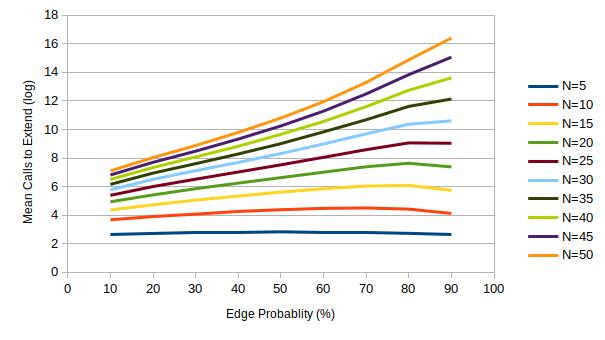
\includegraphics[width=5in]{bron1_calls}
  \caption{Basic Bron Kerbosch algorithm calls to extend.}
  \label{fig:bron1:calls}
\end{figure}

A graph of the \(P=90\%\) values for each order is shown in \figurename~\ref{fig:bron1:runtime}.  This time, the
graph appears to have a log effect and indeed the best curve fit is a mix of \(n\) and \(log(n)\).  This is expected
based on the discussion in \sectionname~\ref{sec:sub:sub:runtime}.  The fit indicates that the runtime complexity is
about \(\BO(2^{0.2259n})\approx\BO(1.17^n)\).

\begin{figure}[H]
  \centering
  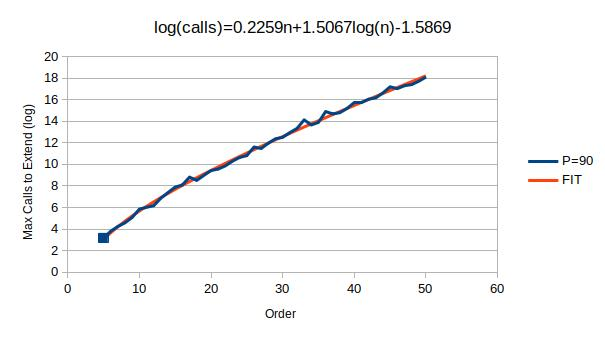
\includegraphics[width=5in]{bron1_runtime}
  \caption{Basic Bron Kerbosch algorithm runtime complexity.}
  \label{fig:bron1:runtime}
\end{figure}

In smart mode, a particular vertex in the \emph{used} list with the smallest number of nonadjacencies to vertices
in the \emph{candidates} list is identified.  The next selected vertex is then a vertex that is not adjacent to the
identified vertex.  This causes the non-maximal bounding condition to occur as soon as possible.
\figurename~\ref{fig:bron2:calls} shows the average number of calls to the \emph{extend} method for the smart
version of the algorithm.

\begin{figure}[H]
  \centering
  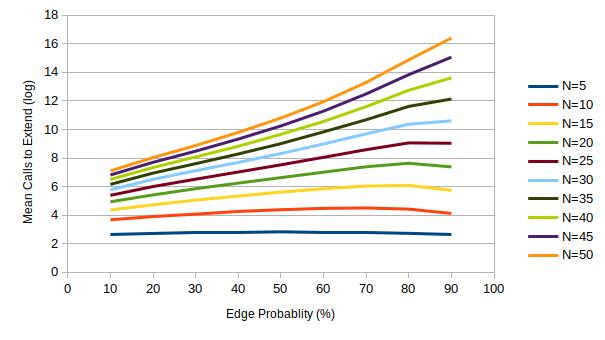
\includegraphics[width=5in]{bron1_calls}
  \caption{Smart Bron Kerbosch algorithm calls to extend.}
  \label{fig:bron2:calls}
\end{figure}

The runtime complexity estimate for the smart version of the algorithm is shown in
\figurename~\ref{fig:bron2:runtime}.  Note that the runtime complexity is improved to
\(\BO(2^{0.1867n})\approx\BO(1.14^n)\).

\begin{figure}[H]
  \centering
  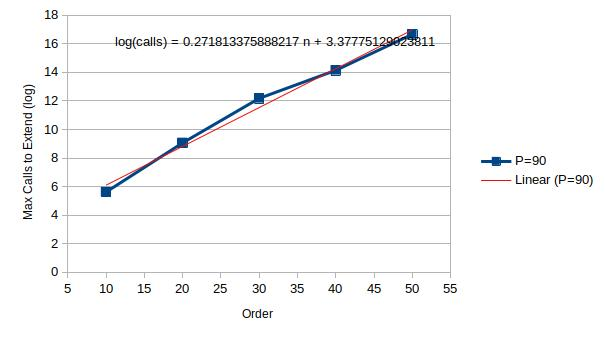
\includegraphics[width=5in]{bron2_runtime}
  \caption{Smart Bron Kerbosch algorithm runtime complexity.}
  \label{fig:bron2:runtime}
\end{figure}

Therefore, BK in smart mode decreases the runtime complexity over the target range from \(\BO(1.17)\) to
\(\BO(1.14)\) and so the improved bounding condition is effective.

\subsection{Finding an Upper Bound}\label{sec:sub:upper}

The most popular technique for finding an upper bound for the chromatic number of a graph is to construct a proper
coloring for the graph using a so-called \emph{sequential} algorithm, often referred to as a \emph{greedy}
algorithm.  The algorithms are sequential because the vertices are ordered in some fashion and are then colored
according to that order.  The algorithms are greedy because a new color is selected whenever one is needed.  The
result is that too many colors may be used; however, such algorithms are P-time and the number of colors used is
suitable as an upper bound for the chromatic number since the graph is at least colorable using that many colors.

The specific steps of a greedy algorithm for a graph \(G\) of order \(n\) are as follows:
\begin{enumerate}
\item Order the vertices in some fashion: \(V=\set{v_1,\ldots,v_n}\).
\item Start with \(C=\emptyset\) and assume some coloring function: \(c:V\to C\).
\item Let \(i=1\).
\item\label{step:greedy:check} Let \(k=\abs{C}\).
\item If \(i=n\) then done and \(k\) is an upper bound for the chromatic number.
\item Determine all of the already colored vertices that are adjacent to \(v_i\):
  \[S=\setb{v_j\in V}{j<i\ \text{and}\ v_iv_j\in E(G)}\]
\item Determine all of the colors used by the vertices in \(S\): \(c[S]\).
\item If \(c[S]=C\) then an additional color is needed for \(v_i\), so add \(c_{k+1}\) to \(C\), let
  \(c_j=c_{k+1}\), and go to step~\ref{step:greedy:color}.
\item Otherwise, an existing color can be reused for \(v_i\) so select \(c_j\) from \(C-c[S]\) with the smallest
  \(j\).
\item\label{step:greedy:color} Color \(v_i\) with \(c_j\) by extending \(c\): \(c(v_i)=c_j\).
\item Let \(i=i+1\).
\item Go to step~\ref{step:greedy:check}.
\end{enumerate}

Indeed, the two most popular theorems used to quickly estimate the chromatic number upper bound of a graph follow
from the worst case result from this algorithm.  The first is based on a random ordering of the
vertices~\cite{chartrand}.

\begin{theorem}
  \label{thm:upper}
  Let \(G\) be a graph.  \(\X(G)\le1+\dmax(G)\)
\end{theorem}

The second, from Welsh and Powell (1967), is based on ordering by non-increasing vertex degree~\cite{welsh}.

\begin{theorem}
  \label{thm:welsh}
  Let \(G\) be a graph:
  \[\X(G)\le\max_i\min\left\{1+\deg(v_i),i\right\}\]
\end{theorem}

Matula, et al.~(1967)~\cite{matula} performed a study on the various well-known chromatic number greedy algorithms
and concluded that ordering the vertices by non-increasing degree order, as in the Welsh Powell bound, worked best.
Matula referred to this algorithm as the \emph{last-first} algorithm.  The results of a random graph analysis of
the last-first greedy algorithm are shown in \figurename~\ref{fig:greedy:error}.  The graph shows the mean
difference between the value found by the greedy algorithm and the actual chromatic number.  Note that the former
is always greater than or equal to the latter.  Due to runtime duration considerations, only \(100\) trials were
run per edge probability and order was limited to \(20\), which is the target range.  The algorithm is exact for an
empty or complete graphs and indeed \figurename~\ref{fig:greedy:error} indicates that the algorithm performs better
at lower and higher edge probabilities.

\begin{figure}[H]
  \centering
  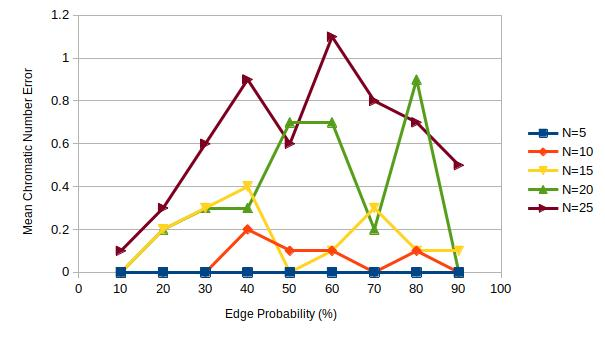
\includegraphics[width=5in]{greedy_error}
  \caption{Last-first greedy algorithm error.}
  \label{fig:greedy:error}
\end{figure}

The mean number of steps is shown in \figurename~\ref{fig:greedy:steps}.  The number of steps increases with both
edge probability and order, so the worst case for each order is assumed to be at \(P=90\%\).

\begin{figure}[H]
  \centering
  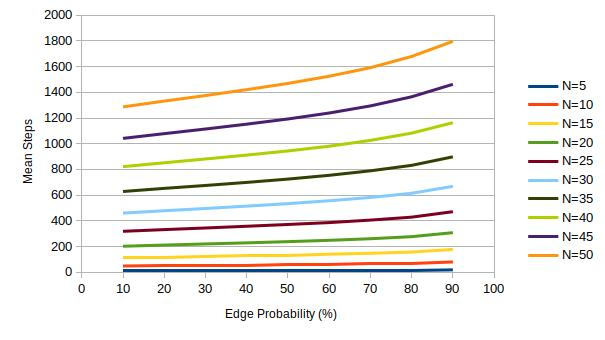
\includegraphics[width=5in]{greedy_steps}
  \caption{Last-first greedy algorithm steps.}
  \label{fig:greedy:steps}
\end{figure}

A graph of the \(P=90\%\) values for each order is shown in \figurename~\ref{fig:greedy:runtime}.  Note that the
runtime complexity is \(\BO(n^2)\) as expected.

\begin{figure}[H]
  \centering
  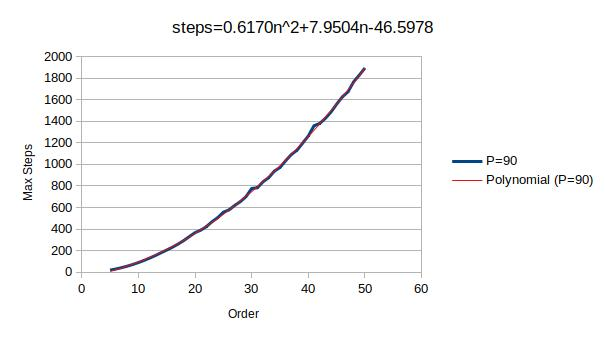
\includegraphics[width=5in]{greedy_runtime}
  \caption{Last-first greedy algorithm runtime complexity.}
  \label{fig:greedy:runtime}
\end{figure}

Matula proposed an improvement to greedy algorithms known as \emph{color interchange}.  Color interchange is based
on the situation summarized by the example in \figurename~\ref{fig:interchange}.  When it is time to color \(v_4\),
the normal greedy algorithm is forced to select a new color.  However, vertices \(v_1\) and \(v_3\) can swap colors
and thus \(v_4\) can use an existing color.

\begin{figure}[H]
  \begin{minipage}{2.5in}
    \centering
    \begin{tikzpicture}[every node/.style={labeled node}]
      \colorlet{c1}{green!25!white}
      \colorlet{c2}{red!25!white}
      \node (4) at (0,0) {\(v_4\)};
      \node [fill=c1] (1) at (2,1) {\(v_1\)};
      \node [fill=c2] (2) at (2,-1) {\(v_2\)};
      \node [fill=c2] (3) at (4,1) {\(v_3\)};
      \draw (4) edge (1) edge (2);
      \draw (1) edge (3);
    \end{tikzpicture}

    Before Swap
  \end{minipage}
  \begin{minipage}{2.5in}
    \centering
    \begin{tikzpicture}[every node/.style={labeled node}]
      \colorlet{c1}{green!25!white}
      \colorlet{c2}{red!25!white}
      \node (4) at (0,0) {\(v_4\)};
      \node [fill=c2] (1) at (2,1) {\(v_1\)};
      \node [fill=c2] (2) at (2,-1) {\(v_2\)};
      \node [fill=c1] (3) at (4,1) {\(v_3\)};
      \draw (4) edge (1) edge (2);
      \draw (1) edge (3);
    \end{tikzpicture}

    After Swap
  \end{minipage}
  \caption{An example that allows color interchange.}
  \label{fig:interchange}
\end{figure}

The specific steps for color interchange when attempting to color vertex \(v_i\) are as follows:
\begin{enumerate}
\item Determine all of the colors that are used for already colored vertices that are adjacent to \(v_i\).
\item Select those colors that occur only once in the neighborhood of \(v_i\).
\item Select all vertices that are already colored with the used-once colors.
\item Construct a subgraph using the selected vertices.
\item\label{step:color:part} Partition the subgraph into components.
\item Find a component that includes one vertex and excludes one vertex that is adjacent to \(v_i\) in the original
  graph.  If no such component is found then interchange is not possible and a new color must be used for \(v_i\).
\item Let \(c_1\) be the color of the included vertex and let \(c_2\) be the color of the excluded vertex.
\item Interchange colors \(c_1\) and \(c_2\) for all such colored vertices in the selected component.
\item Color \(c_1\) is now available for \(v_i\).
\end{enumerate}

The mean error when color interchange is added to the last-first greedy algorithm is shown in
\figurename~\ref{fig:greedyint:error}.  The Hopcroft Tarjan algorithm~\cite{hopcroft} introduced in
\sectionname~\ref{sec:sub:sub:impact} was used to partition the subgraph in step~\ref{step:color:part}.  The
algorithm still tends to do better at lower and higher edge densities.  It appears that color interchange has a
slight advantage at higher orders.

\begin{figure}[H]
  \centering
  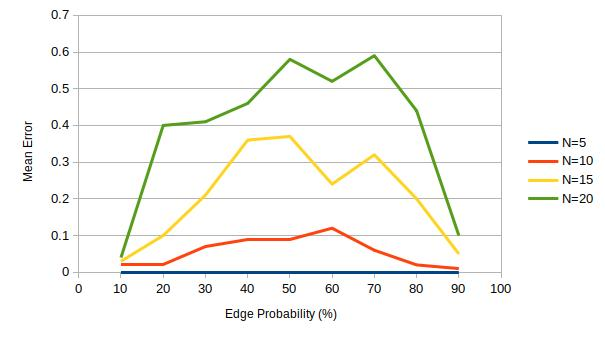
\includegraphics[width=5in]{greedyint_error}
  \caption{Last-first greedy algorithm with color interchange error.}
  \label{fig:greedy:error}
\end{figure}

The mean number of steps with interchange is shown in \figurename~\ref{fig:greedyint:steps}.  Once again, the
number of steps increases with both edge probability and order, so the worst case for each order is assumed to be
at \(P=90\%\).

\begin{figure}[H]
  \centering
  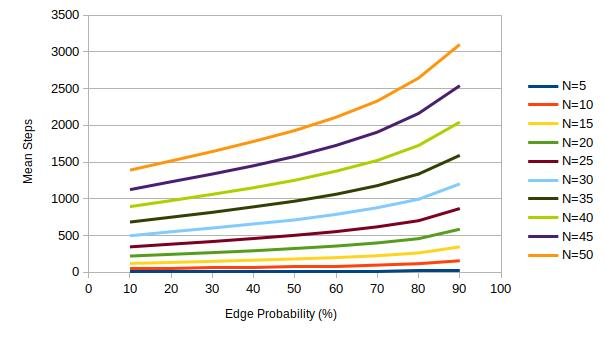
\includegraphics[width=5in]{greedyint_steps}
  \caption{Last-first greedy algorithm with color interchange steps.}
  \label{fig:greedyint:steps}
\end{figure}

A graph of the \(P=90\%\) values for each order is shown in \figurename~\ref{fig:greedyint:runtime}.  Note that
color interchange is a bit expensive; however, the runtime complexity is still\(\BO(n^2)\).

\begin{figure}[H]
  \centering
  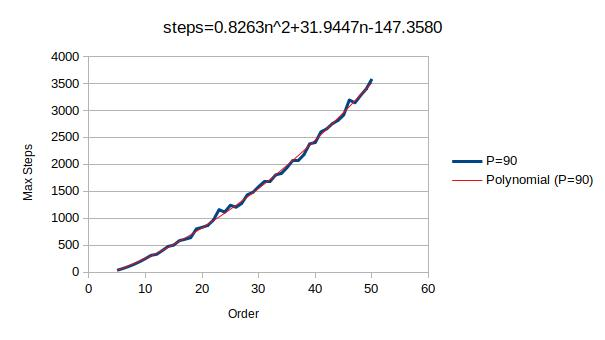
\includegraphics[width=5in]{greedyint_runtime}
  \caption{Last-first greedy algorithm with color interchange runtime complexity.}
  \label{fig:greedyint:runtime}
\end{figure}

\subsection{The Christofides Algorithm}\label{sec:sub:christofides}

The first exhaustive algorithm that will be examined was proposed by Cypriot mathematician Nicos
Christofides~(1971)~\cite{christofides}.  The Christofides algorithm is a breadth-first algorithm that assembles
maximal independent sets from a graph until the first combination that uses all of the vertices is found.  Thus,
the Bron Kerbosch algorithm is a vital part of the Christofides algorithm.

The Christofides algorithm starts by decomposing a graph \(G\) into all of its maximal independent sets.  This
constitutes the first level of the state tree.  Then, for each maximal independent set with vertices \(S\), the
subgraph \(G-S\) is constructed and all of its maximal independent sets are found.  Each of these sets is combined
with the previous maximal independent sets to form the next layer of the state tree.  This process continues until
the first time that all of the vertices in \(G\) are used.  The number of maximal independent sets used to form the
final combination is the chromatic number.

The Christofides does have bounding conditions.  If the vertices in any new combination of maximal independent sets
is a subset of a previous combination then the subtree for the latter is pruned.  If the former is a subset of the
latter then the former subtree is pruned by replacing its state with the state of the latter.

For example, consider the graph in \figurename~\ref{fig:cfexample}.

\begin{figure}[H]
  \centering
  \begin{tikzpicture}
    \cycleNnodes{5}{(0,0)}{0.75in}{90}{c};
    \begin{scope}[every node/.style={labeled node}]
      \node (1) at (c1) {\(1\)};
      \node (2) at (c2) {\(2\)};
      \node (3) at (c3) {\(3\)};
      \node (4) at (c4) {\(4\)};
      \node (5) at (c5) {\(5\)};
    \end{scope}
    \draw (1) edge (2) edge (3) edge (4) edge (5);
    \draw (2) edge (3);
    \draw (3) edge (4);
    \draw (4) edge (5);
  \end{tikzpicture}
  \caption{A Christofides algorithm example.}
  \label{fig:cfexample}
\end{figure}

The Bron Kerbosch algorithm is used to decompose \figurename~\ref{fig:cfexample} into the maximal independent sets
\(\set{1}\), \(\set{2,4}\), \(\set{2,5}\), and \(\set{3,5}\).  This first level is shown in
\figurename~\ref{fig:cflevel1}, along with the resulting subgraphs.

\begin{figure}[H]
  \begin{minipage}{1.5in}
    \centering
    \((1)\)

    \bigskip

    \begin{tikzpicture}
      \cycleNnodes{5}{(0,0)}{0.5in}{90}{c};
      \begin{scope}[every node/.style={labeled node}]
        \node (2) at (c2) {\(2\)};
        \node (3) at (c3) {\(3\)};
        \node (4) at (c4) {\(4\)};
        \node (5) at (c5) {\(5\)};
      \end{scope}
      \draw (2) edge (3);
      \draw (3) edge (4);
      \draw (4) edge (5);
    \end{tikzpicture}
  \end{minipage}
  \begin{minipage}{1.25in}
    \centering
    \((2,4)\)

    \bigskip

    \begin{tikzpicture}
      \cycleNnodes{5}{(0,0)}{0.5in}{90}{c};
      \begin{scope}[every node/.style={labeled node}]
        \node (1) at (c1) {\(1\)};
        \node (3) at (c3) {\(3\)};
        \node (5) at (c5) {\(5\)};
      \end{scope}
      \draw (1) edge (3) edge (5);
    \end{tikzpicture}
  \end{minipage}
  \begin{minipage}{1.25in}
    \centering
    \((2,5)\)

    \bigskip

    \begin{tikzpicture}
      \cycleNnodes{5}{(0,0)}{0.5in}{90}{c};
      \begin{scope}[every node/.style={labeled node}]
        \node (1) at (c1) {\(1\)};
        \node (3) at (c3) {\(3\)};
        \node (4) at (c4) {\(4\)};
      \end{scope}
      \draw (1) edge (3) edge (4);
      \draw (3) edge (4);
    \end{tikzpicture}
  \end{minipage}
  \begin{minipage}{1.25in}
    \centering
    \((3,5)\)

    \bigskip

    \begin{tikzpicture}
      \cycleNnodes{5}{(0,0)}{0.5in}{90}{c};
      \begin{scope}[every node/.style={labeled node}]
        \node (1) at (c1) {\(1\)};
        \node (2) at (c2) {\(2\)};
        \node (4) at (c4) {\(4\)};
      \end{scope}
      \draw (1) edge (2) edge (4);
    \end{tikzpicture}
  \end{minipage}
  \caption{Level 1 of a Christofides algorithm example.}
  \label{fig:cflevel1}
\end{figure}

The next level starts with the leftmost subgraph in \figurename~\ref{fig:cflevel1}.  It has the maximal independent
sets \(\set{2,4}\) and \(\set{3,5}\).  These are combined with the parent state to form the next states
\(\set{\set{1},\set{2,4}}\) and \(\set{\set{1},\set{3,5}}\).  Likewise, the second graph in
\figurename~\ref{fig:cflevel1} contains maximal independent sets \(\set{1}\) and \(\set{3,5}\).  This yields the
next states \(\set{\set{2,4},\set{1}}\) and \(\set{\set{2,4},\set{3,5}}\); however, the vertices in
\(\set{\set{2,4},\set{1}}\) are a subset of the previous state \(\set{\set{1},\set{2,4}}\) and so the new subtree
is pruned.  This process continues for the third and fourth subgraph in \figurename~\ref{fig:cflevel1}.  The second
level results are as follows:

\begin{tabular}{ccccccccc}
  \((1|24)\) & \((1|35)\) & \(\cancel{(24|1)}\) & \((24|35)\) & \((25|1)\) & \(\cancel{(25|3)}\) &
  \(\cancel{(25|4)}\) & \(\cancel{(35|1)}\) & \(\cancel{(35|24)}\)
\end{tabular}

Next, the first state in the second level contains a single maximal independent set \(\set{3,5}\), which when
combined with the parent state uses all of the vertices.  The final coloring is thus \((1|24|35)\) and the graph is
\chromatic{3} as shown in \figurename~\ref{fig:cfresults}.

\begin{figure}[H]
  \centering
  \begin{tikzpicture}
    \colorlet{clr1}{red!25!white}
    \colorlet{clr2}{green!25!white}
    \colorlet{clr3}{blue!25!white}
    \cycleNnodes{5}{(0,0)}{0.75in}{90}{c};
    \begin{scope}[every node/.style={labeled node}]
      \node [fill=clr1] (1) at (c1) {\(1\)};
      \node [fill=clr2] (2) at (c2) {\(2\)};
      \node [fill=clr3] (3) at (c3) {\(3\)};
      \node [fill=clr2] (4) at (c4) {\(4\)};
      \node [fill=clr3] (5) at (c5) {\(5\)};
    \end{scope}
    \draw (1) edge (2) edge (3) edge (4) edge (5);
    \draw (2) edge (3);
    \draw (3) edge (4);
    \draw (4) edge (5);
  \end{tikzpicture}
  \caption{Christofides algorithm example results.}
  \label{fig:cfresults}
\end{figure}

The results of a random graph analysis of the Christofides algorithm are shown in \figurename~\ref{fig:cfstates}.
The graph shows edge probability versus the mean of the number of states for graphs of increasing order with
\(1000\) trials per edge for orders less than \(20\) and \(100\) trials per edge for orders greater than or equal
to \(20\) (due to increased runtime duration).

\begin{figure}[H]
  \centering
  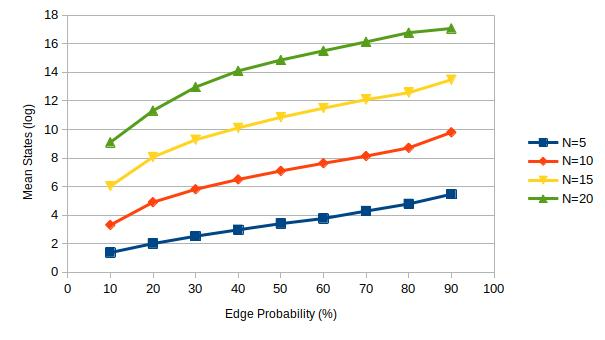
\includegraphics[width=5in]{christofides_states}
  \caption{Christofides algorithm mean number of states.}
  \label{fig:cfstates}
\end{figure}

The number of states increases with both graph order and edge probability.  The worst case for each order is thus
assumed to occur at \(90\%\) edge probability.  A log (base 2) plot of the maximum number of states for each order
at \(90\%\) edge probability is plotted in \figurename~\ref{fig:cfruntime}.  A logarithmic curve fit is used to
approximate the runtime complexity for the algorithm.  The curve fit indicates that the runtime complexity is about
\(\BO(2^{9.2127\ln(n)})\approx\BO(2^{6.7858\log(n)})\approx\BO(84^{\log(n)})\) --- still not polynomial but better
than exponential.

\begin{figure}[H]
  \centering
  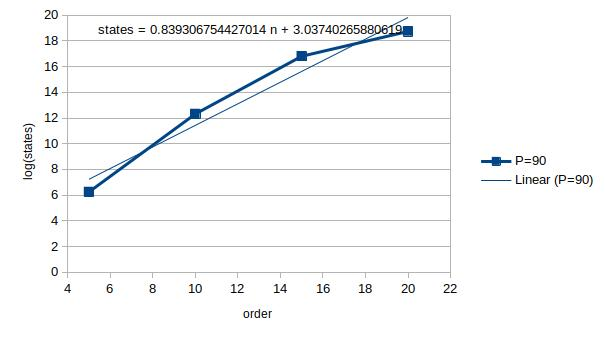
\includegraphics[width=5in]{christofides_runtime}
  \caption{Christofides algorithm runtime complexity assuming \(\BO(c^n)\).}
  \label{fig:cfruntime}
\end{figure}

One drawback of the Christofides algorithm is the fact that each level must be maintained entirely in memory before
moving on to the next level.  As has been show, the breadth of state graphs grows exponentially, so depth-first
algorithms are generally preferred.  Wang~(1974)~\cite{wang} proposes two improvements to the Christofides
algorithm to combat this memory usage.  The first improvement prunes a large number of subtrees and the second
improvement converts the algorithm to a depth-first search.

Wang's first proposal is based on \lemmaname~\ref{lem:wang}

\begin{lemma}
  \label{lem:wang}
  Let \(G\) be a graph, let \(v\in V(G)\), and let \(\set{M_1,\ldots,M_r}\) be all of the maximal independent sets
  in \(G\) containing \(v\).  There exists a chromatic coloring of \(G\) containing one of the \(M_i\).
\end{lemma}

\begin{proof}
  Assume that \(G\) is \chromatic{k} and let \(\set{A_1,\ldots,A_k}\) be the independent sets of a chromatic
  coloring of \(G\).  Assume without loss of generality (AWLOG) that \(v\in A_1\).  It must be the case that
  \(A_1\subseteq M_i\) for some \(1\le i\le r\), since all of the \(M_i\) are maximal.  Now, let \(X=M_i-A_1\) and
  let \(X_j=A_j-X\) for \(2\le j\le k\).  Next, construct the coloring \(\set{M_i,X_2,\ldots,X_k}\).  This is a
  \chromatic{k} coloring of \(G\) containing \(M_i\).
\end{proof}

Basically, \lemmaname~\ref{lem:wang} says that any independent set in a chromatic coloring of a graph \(G\)
containing a vertex \(v\) can be extended to a maximal independent set containing \(v\) by snatching vertices from
the other independent sets in the coloring.

Next consider the fact that each state in the Christofides algorithm state tree represents a subgraph and the goal
is to (recursively) find a chromatic coloring for that subgraph.  Therefore, a particular vertex can be selected
and only MISs containing that vertex need be considered for the next level.  So, at each state, select the vertex
that appears in the fewest MISs of the subgraph; the subtrees corresponding to the MISs that do not contain the
selected vertex are pruned.

Referring back to the example in \figurename~\ref{fig:cfexample}, recall that the first level MISs were:
\(\set{1}\), \(\set{2,4}\), \(\set{2,5}\), and \(\set{3,5}\).  Vertices \(1\), \(3\), and \(4\) occur in only
one MIS each.  So if \(1\) is selected, only the leftmost subgraph in \figurename~\ref{fig:cflevel1} need be
considered.

Wang's second improvement is to convert the search to a depth-first search, keeping track of the minimum length
branch from the root state to a leaf state.  Branches that equal or exceed the current minimum are pruned.
Branches that are smaller than the current minimum become the new current minimum.  Although this does require that
the entire pruned tree be traversed, the hope is that the first improvement has pruned enough subtrees so that the
depth-first search is now economical.

The results of a random graph analysis of Wang's improvements to the Christofides algorithm are shown in
\figurename~\ref{fig:wangstates}.  The graph shows edge probability versus the mean of the number of states for
graphs of increasing order with \(1000\) trials per edge for orders less than \(20\) and \(100\) trials per edge
for orders greater than or equal to \(20\) (due to increased runtime duration).

\begin{figure}[H]
  \centering
  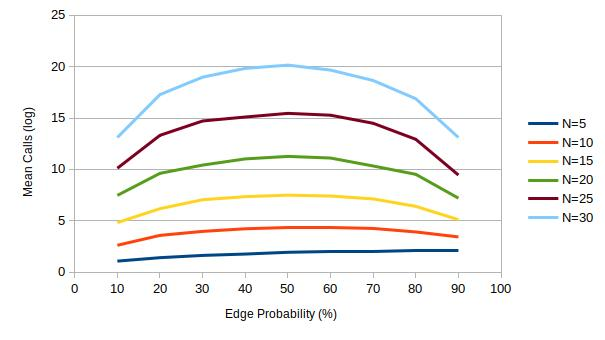
\includegraphics[width=5in]{wang_calls}
  \caption{Christofides algorithm with Wang improvements mean number of states.}
  \label{fig:wangstates}
\end{figure}

The results are quite surprising.  Not only is there a dramatic overall improvement, it now appears that the worst
case occurs at moderate edge density.  Intuition suggests that lower edge density graphs will have fewer and larger
MISs.  For the high density case, it may be that each vertex is in fewer MISs.  The worst case for each order is
thus assumed to occur at \(50\%\) edge probability.  A log (base 2) plot of the maximum number of states for each
order at \(50\%\) edge probability is plotted in \figurename~\ref{fig:wangruntime}.  This time, a polynomial curve
fit appears to be more appropriate.  The curve fit indicates that the runtime complexity is about
\(\BO(2^{0.0083n^2})\approx\BO(1.0057^{n^2})\).

\begin{figure}[H]
  \centering
  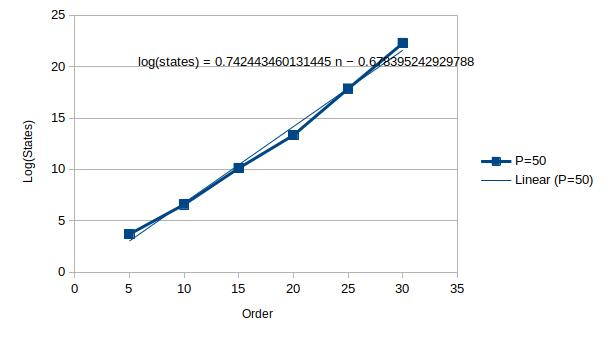
\includegraphics[width=5in]{wang_runtime}
  \caption{Christofides algorithm with Wang improvements runtime complexity.}
  \label{fig:wangruntime}
\end{figure}

A comparison of the Christofides and Wang runtime complexities indicates some pitfalls of big-\(\BO\) notation and
improvements to exhaustive algorithms.  The \(\BO(c^{\log(n)})\) runtime complexity of Christofides versus the
\(\BO(c^{n^2})\) runtime complexity of Wang indicates that for large \(n\) the benefits of the Wang improvements
are lost to the required additional processing.  Comparing the two fit equations from \figurename~\ref{fig:cfruntime}
and \figurename~\ref{fig:wangruntime}, the break even point appears to be \(n\approx30\).

\subsection{Zykov Algorithms}\label{sec:sub:zykov}

The second exhaustive algorithm that will be examined is based on a branching technique attributed to Ukranian
mathematician Alexandre A. Zykov.  In his 1949 paper (translated by the AMS in 1952)~\cite{zykov}, Zykov addresses
the question: given a graph \(G\) and a number \(k\in\N\), how many ways are there to properly color \(G\) using at
most \(k\) colors?  In fact, he is not particularly concerned about the chromatic number, which he calls the
\emph{rank} of a graph.

To solve this problem, Zykov notes that in any proper coloring of a graph:
\begin{enumerate}
\item Nonadjacent vertices have either the same color or different colors.
\item Adjacent vertices always have different colors.
\end{enumerate}
If nonadjacent vertices have the same color then they can be contracted and the resulting graph retains the same
\coloring{k} as the original graph.  This is demonstrated in \figurename~\ref{fig:zvcon}.

\begin{figure}[H]
  \begin{minipage}{2.5in}
    \centering
    \begin{tikzpicture}[every node/.style={labeled node}]
      \colorlet{c1}{green!25!white}
      \colorlet{c2}{blue!25!white}
      \colorlet{c3}{red!25!white}
      \node (d) [fill=c2] at (0,0) {\(d\)};
      \node (c) [fill=c3,right=of d] {\(c\)};
      \node (b) [fill=c2,above=of c] {\(b\)};
      \node (a) [fill=c1,above=of d] {\(a\)};
      \draw (a) -- (b);
      \draw (a) -- (c) -- (d) -- (a);
    \end{tikzpicture}

    \(G\)
  \end{minipage}
  \begin{minipage}{2.5in}
    \centering
    \begin{tikzpicture}[every node/.style={labeled node}]
      \colorlet{c1}{green!25!white}
      \colorlet{c2}{blue!25!white}
      \colorlet{c3}{red!25!white}
      \node (bd) [fill=c2] at (0,0) {\(bd\)};
      \node (c) [fill=c3,right=of bd] {\(c\)};
      \node (a) [fill=c1,above=of bd] {\(a\)};
      \draw (a) -- (c) -- (bd) -- (a);
    \end{tikzpicture}

    \(G\cdot bd\)
  \end{minipage}
  \caption{Same colors with vertex contraction.}
  \label{fig:zvcon}
\end{figure}

If nonadjacent vertices have different colors then they can be joined by an edge and the resulting graph retains
the same \coloring{k} as the original graph.  This is demonstrated in \figurename~\ref{fig:zeadd}.

\begin{figure}[H]
  \begin{minipage}{2.5in}
    \centering
    \begin{tikzpicture}[every node/.style={labeled node}]
      \colorlet{c1}{green!25!white}
      \colorlet{c2}{blue!25!white}
      \colorlet{c3}{red!25!white}
      \node (d) [fill=c2] at (0,0) {\(d\)};
      \node (c) [fill=c3,right=of d] {\(c\)};
      \node (b) [fill=c2,above=of c] {\(b\)};
      \node (a) [fill=c1,above=of d] {\(a\)};
      \draw (a) -- (b);
      \draw (a) -- (c) -- (d) -- (a);
    \end{tikzpicture}

    \(G\)
  \end{minipage}
  \begin{minipage}{2.5in}
    \centering
    \begin{tikzpicture}[every node/.style={labeled node}]
      \colorlet{c1}{green!25!white}
      \colorlet{c2}{blue!25!white}
      \colorlet{c3}{red!25!white}
      \node (d) [fill=c2] at (0,0) {\(d\)};
      \node (c) [fill=c3,right=of d] {\(c\)};
      \node (b) [fill=c2,above=of c] {\(b\)};
      \node (a) [fill=c1,above=of d] {\(a\)};
      \draw (a) -- (b) -- (c);
      \draw (a) -- (c) -- (d) -- (a);
    \end{tikzpicture}

    \(G+bc\)
  \end{minipage}
  \caption{Different colors with edge addition.}
  \label{fig:zeadd}
\end{figure}

By applying these steps recursively, all of the possible partitions of the nonadjacent vertices to independent sets
are generated.  The termination condition for each recursive path is a complete graph of some varying order \(k\).
Each node in the complete graph represents an independent set of nonadjacent nodes in the original graph that have
been combined via vertex contraction.  Thus, each complete graph of order \(k\) represents a possible \coloring{k}
of the original graph.  The complete graphs of smallest order represent chromatic colorings and their order is the
chromatic number of the original graph.

Zykov uses a graph equation syntax to record the recursive processing of a graph, where each line in the equation
represents the next recursive layer.  Isomorphic graphs are combined with a frequency multiplier at each layer.
This is demonstrated in \figurename~\ref{fig:greqn}.

\begin{figure}[H]
  \begin{align*}
    \begin{minipage}{0.75in}
      \centering
      \begin{tikzpicture}[every node/.style={unlabeled node}]
        \node (a1) at (0,0) {};
        \node (a2) [right=of a1] {};
        \node (a3) [above=of a2] {};
        \node (a4) [above=of a1] {};
        \draw (a3) -- (a4) -- (a1) -- (a2) -- (a4);
      \end{tikzpicture}
    \end{minipage} &=
    \begin{minipage}{0.75in}
      \centering
      \begin{tikzpicture}[every node/.style={unlabeled node}]
        \node (b1) at (0,0) {};
        \node (b2) [above=of b1] {};
        \node (b3) [right=of b1] {};
        \draw (b1) -- (b2) -- (b3) -- (b1);
      \end{tikzpicture}
    \end{minipage} +
    \begin{minipage}{0.75in}
      \centering
      \begin{tikzpicture}[every node/.style={unlabeled node}]
        \node (c1) at (0,0) {};
        \node (c2) [right=of a1] {};
        \node (c3) [above=of a2] {};
        \node (c4) [above=of a1] {};
        \draw (c2) -- (c3) -- (c4) -- (c1) -- (c2) -- (c4);
      \end{tikzpicture}
    \end{minipage} \\
    &= \begin{minipage}{0.75in}
      \centering
      \begin{tikzpicture}[every node/.style={unlabeled node}]
        \node (b1) at (0,0) {};
        \node (b2) [above=of b1] {};
        \node (b3) [right=of b1] {};
        \draw (b1) -- (b2) -- (b3) -- (b1);
      \end{tikzpicture}
    \end{minipage} +
    \begin{minipage}{0.75in}
      \centering
      \begin{tikzpicture}[every node/.style={unlabeled node}]
        \node (b1) at (0,0) {};
        \node (b2) [above=of b1] {};
        \node (b3) [right=of b1] {};
        \draw (b1) -- (b2) -- (b3) -- (b1);
      \end{tikzpicture}
    \end{minipage} +
    \begin{minipage}{0.75in}
      \centering
      \begin{tikzpicture}[every node/.style={unlabeled node}]
        \node (c1) at (0,0) {};
        \node (c2) [right=of a1] {};
        \node (c3) [above=of a2] {};
        \node (c4) [above=of a1] {};
        \draw (c2) -- (c3) -- (c4) -- (c1) -- (c2) -- (c4);
        \draw (c1) -- (c3);
      \end{tikzpicture}
    \end{minipage} \\
    &= 2
    \begin{minipage}{0.75in}
      \centering
      \begin{tikzpicture}[every node/.style={unlabeled node}]
        \node (b1) at (0,0) {};
        \node (b2) [above=of b1] {};
        \node (b3) [right=of b1] {};
        \draw (b1) -- (b2) -- (b3) -- (b1);
      \end{tikzpicture}
    \end{minipage} +
    \begin{minipage}{0.75in}
      \centering
      \begin{tikzpicture}[every node/.style={unlabeled node}]
        \node (c1) at (0,0) {};
        \node (c2) [right=of a1] {};
        \node (c3) [above=of a2] {};
        \node (c4) [above=of a1] {};
        \draw (c2) -- (c3) -- (c4) -- (c1) -- (c2) -- (c4);
        \draw (c1) -- (c3);
      \end{tikzpicture}
    \end{minipage} \\
    &= 2K_3+K_4
  \end{align*}
  \caption{A Zykov graph equation example.}
  \label{fig:greqn}
\end{figure}

Determining whether two graphs are isomorphic is hard, so combining isomorphic graphs in all but the very simple
cases should be skipped; the complete graphs resulting from the further processing of two isomorphic graphs will
eventually be combined anyway by the end.

Zykov was trying to determine the number of \coloring{k}s of a graph without color indifference: each permutation
of colors for a particular distribution is considered unique.  Thus, Zykov multiplied each complete graph
coefficient in the final line of a graph equation by the number of permutations resulting from selecting the order
\(n\) of the particular complete graph from \(k\) colors:
\[k^{(n)}=k(k-1)(k-2)\cdots(k-n+1)\]
So the total number of unique colorings for the example shown in \figurename~\ref{fig:greqn} using \(k\) colors would
be:
\begin{equation}
  \label{eqn:cpfact}
  M(G,k)=2k^{(3)}+k^{(4)}
\end{equation}
\equationname~\ref{eqn:cpfact} is known as the \emph{factorial form} of the \emph{chromatic polynomial} for the
graph.  The corresponding \emph{expanded form} is shown in \equationname~\ref{eqn:cpexp}.
\begin{equation}
  \label{eqn:cpexp}
  M(G,k)=k^4-4k^3+5k^2-2k
\end{equation}

Read~(1968)~\cite{read} expands on the construction of the factorial form of the chromatic polynomial for a graph
and proves several theorems regarding the expanded form.  Some examples are:
\begin{enumerate}
\item \(M(G,k)=M(G\cdot uv)+M(G+uv)\), where \(u\) and \(v\) are any two nonadjacent vertices in the current
  recursive step.
\item The degree of M(G,k) is the order of \(G\).
\item The highest order coefficient is \(1\).
\item There is no constant term.
\item The terms alternate in sign.
\end{enumerate}
In fact, Read shows that the expanded form is actually an inclusion-exclusion equation resulting from starting with
all possible proper and improper colorings \(k^n\) and then subtracting the improper colorings.

Corneil and Graham~(1973) extend Zykov's work with \theoremname~\ref{thm:corneil}~\cite{corneil}:

\begin{theorem}
  \label{thm:corneil}
  Let \(G\) be a graph and let \(u\) and \(v\) be two nonadjacent vertices in \(G\):
  \[\X(G)=\min\set{\X(G\cdot uv),\X(G+uv)}\]
\end{theorem}

Zykov's method combined with \theoremname~\ref{thm:corneil} can be used to construct a depth-first branching
algorithm for finding the chromatic number and a chromatic coloring for a graph \(G\).  Each state in the state
tree for such an algorithm is represented by a graph whose nodes are sets of contracted vertices from \(G\) and
hence represent independent sets in a candidate coloring, and whose edges are the edges remaining after the vertex
contractions.  The leaves of the state tree are complete graphs that represent proper colorings.  The leaf state
graphs with the smallest order are chromatic colorings.  Such a state tree is called a \emph{Zykov tree} and a
branch (and bound) algorithm that uses such trees is called a \emph{Zykov algorithm}~\cite{corneil}.

The Zykov tree for the example in \figurename~\ref{fig:greqn} is shown in \figurename~\ref{fig:ztree}.  Note that
the three leaf states are complete graphs of order \(3\) or \(4\).  Therefore, the example in
\figurename~\ref{fig:greqn} is \chromatic{3} and the two \(K_3\) leaves represent chromatic colorings.

\begin{figure}[H]
  \centering
  \begin{tikzpicture}
    \node (a) [draw,circle] at (0,0) {
      \begin{tikzpicture}[every node/.style={unlabeled node}]
        \node (a1) at (0,0) {};
        \node (a2) [right=of a1] {};
        \node (a3) [above=of a2] {};
        \node (a4) [above=of a1] {};
        \draw (a3) -- (a4) -- (a1) -- (a2) -- (a4);
      \end{tikzpicture}
    };
    \node (b) [draw,circle,below left=of a] {
      \begin{tikzpicture}[every node/.style={unlabeled node}]
        \node (b1) at (0,0) {};
        \node (b2) [above=of b1] {};
        \node (b3) [right=of b1] {};
        \draw (b1) -- (b2) -- (b3) -- (b1);
      \end{tikzpicture}
    };
    \node (c) [draw,circle,below right=of a] {
      \begin{tikzpicture}[every node/.style={unlabeled node}]
        \node (c1) at (0,0) {};
        \node (c2) [right=of a1] {};
        \node (c3) [above=of a2] {};
        \node (c4) [above=of a1] {};
        \draw (c2) -- (c3) -- (c4) -- (c1) -- (c2) -- (c4);
      \end{tikzpicture}
    };
    \node (d) [draw,circle,below left=of c] {
      \begin{tikzpicture}[every node/.style={unlabeled node}]
        \node (d1) at (0,0) {};
        \node (d2) [above=of d1] {};
        \node (d3) [right=of d1] {};
        \draw (d1) -- (d2) -- (d3) -- (d1);
      \end{tikzpicture}
    };
    \node (e) [draw,circle,below right=of c] {
      \begin{tikzpicture}[every node/.style={unlabeled node}]
        \node (c1) at (0,0) {};
        \node (c2) [right=of a1] {};
        \node (c3) [above=of a2] {};
        \node (c4) [above=of a1] {};
        \draw (c2) -- (c3) -- (c4) -- (c1) -- (c2) -- (c4);
        \draw (c1) -- (c3);
      \end{tikzpicture}
    };
    \draw (a) edge (b) edge (c);
    \draw (c) edge (d) edge (e);
  \end{tikzpicture}
  \caption{A Zykov tree example.}
  \label{fig:ztree}
\end{figure}

The worst case for a Zykov algorithm with no bounding is an empty graph, where the number of leaf nodes is
equivalent to the number of partitions of the set of vertices.  This is known to be the so-called Bell
number~\cite{graham}:
\[B_n=\sum_{k=1}^nS_{n,k}\]
where the \(S_{n,k}\) are the so-called Stirling numbers of the second kind:
\[S_{n,k}=\frac{1}{k!}\sum_{i=0}^k(-1)^i\binom{k}{i}(k-i)^n\]
The actual runtime complexity is worse because each partition leaf node is at the end of a branch from the root
state consisting of a certain number of states that depends on the number of nonadjacencies in a graph.

Branch-and-bound Zykov algorithms require the following components:
\begin{enumerate}
\item A main routine that establishes \(G\) as the root of the state tree.
\item A global variable \(X\) that records the state corresponding to the current smallest \coloring{k}.
\item A global variable \(b\) that records the current upper bound for the chromatic number of \(G\).
\item A method to determine a lower bound for the chromatic number of a graph.
\item A method to determine an upper bound \(k\) for the chromatic number of a graph \(G\) and a corresponding
  \coloring{k} of \(G\).
\item A recursive subroutine that performs the depth-first search of the state tree and updates \(X\) and \(b\) as
  necessary.
\end{enumerate}

The lower bound method is typically one of the clique number lower bound algorithms (e.g. Edwards Elphick).  The
upper bound method is typically a greedy coloring algorithm (e.g., last-first).

The steps of the main routine are as follows:
\begin{enumerate}
\item Construct a graph \(G'\) that is isomorphic to \(G\) and where each vertex in \(G'\) is a set of contracted
  vertices initialized to a one element set containing the corresponding vertex in \(G\).
\item Run the greedy algorithm and set \(X\) and \(b\) based on the results.
\item Call the recursive subroutine with \(G'\).
\item Return \(b\) or \(n(X)\) as the found chromatic number for \(G\) and \(X\) representing a chromatic coloring
  of \(G\).
\end{enumerate}

The recursive subroutine is called with a graph \(H\) and has access to \(X\) and \(b\).  The steps are as follows:
\begin{enumerate}
\item If \(n(H)<b\) then \(b=n(H)\).
\item If \(H\) is not complete then go to step~\ref{step:zbound:branch}.
\item If \(n(H)<n(X)\) then \(X=H\).
\item Go to step~\ref{step:zbound:done}.
\item Determine the chromatic number lower bound for \(H\).  If it is greater than or equal to the current
  upper bound then go to step~\ref{step:zbound:done}.
\item\label{step:zbound:branch} Select any two nonadjacent vertices \(u\) and \(v\) in \(H\).
\item Construct \(H'=H\cdot uv\), where the vertex set for the new contracted vertex is the union of the vertex
  sets for \(u\) and \(v\).
\item Recursively call this subroutine with \(H'\).
\item Construct \(H''=H+uv\).
\item Recursively call this subroutine with \(H''\).
\item\label{step:zbound:done} Return.
\end{enumerate}

McDiarmid~(1978)~\cite{mcdiarmid} predicts that even with bounding, Zykov algorithms have a runtime complexity of
\(\BO(c^{n\sqrt{\log(n)}})\) for some real number constant \(c>1\), which is worse than exponential.  Thus Zykov
algorithms will generally perform worse than Christofides-type algorithms.

\subsection{The Corneil Graham Algorithm}\label{sec:sub:corneil}

This section examines a well-known example of a Zykov algorithm proposed by Corneil and
Graham~(1973)~\cite{corneil}.
